\section{Objective Functions for MSA}
\label{sec:objective _function}
There are numerous objective functions defined for MSA in the literature. We identify the following widely used objective functions from the recent works and briefly discuss their feasibility in MSA:

\begin{itemize}
	
	\item \textbf{Maximize sum of pairs score}~\cite{seeluangsawat2005multiple, da2010alineaga}:  
	This is an extension of pairwise sequence alignment score. Pairwise score is calculated for each pair of aligned sequences. Then, we calculate the total score by summing pairwise scores of all possible pairs. In Figure \ref{fig:pairwise}, the pairwise score is calculated by considering the elements of the same columns of two aligned sequences with the scoring or substitution matrix $\delta$. There are some standard substitution matrices for biological sequences at~\url{ftp://ftp.ncbi.nih.gov/blast/matrices/}.
	
	
	\begin{figure}[!htbp]
		\begin{adjustwidth}{-0.2cm}{}
			\centering
			\begin{subfigure}[b]{0.5\columnwidth}
				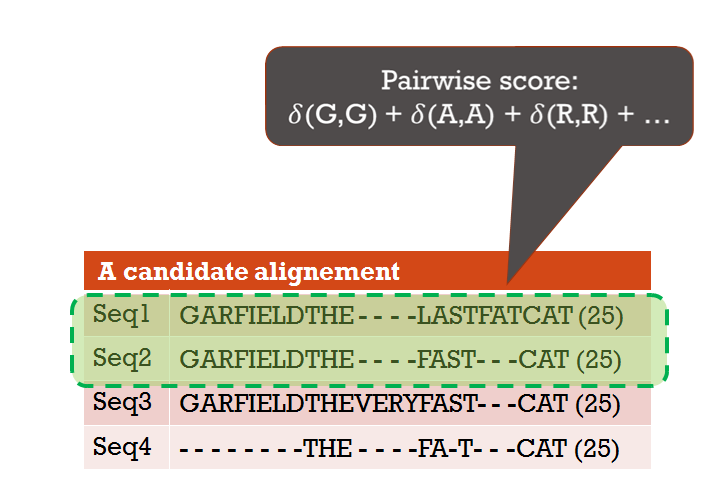
\includegraphics[width=\columnwidth]{Figure/pairwise}
				\caption{Pairwise score of two aligned sequences.}
				\label{fig:pairwise}
			\end{subfigure}	
			\begin{subfigure}[b]{0.5\columnwidth}
				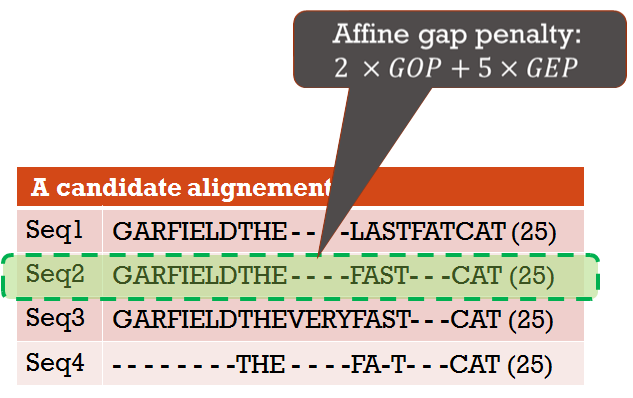
\includegraphics[width=\columnwidth]{Figure/agp}
				\caption{Affine gap penalty of an aligned sequence.}
				\label{fig:agp}
			\end{subfigure}
			\begin{subfigure}[b]{0.5\columnwidth}
				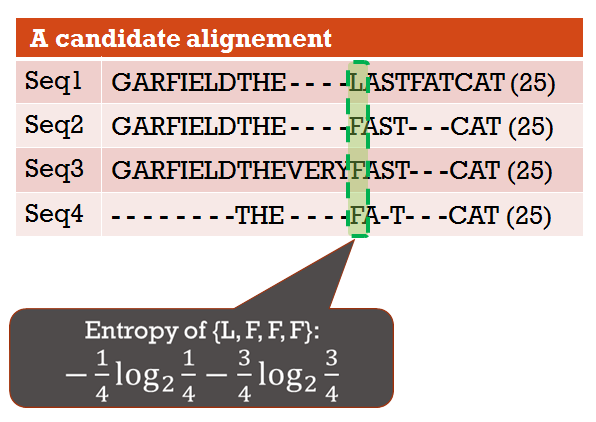
\includegraphics[width=\columnwidth]{Figure/entropy_score}
				\caption{Entropy of a column of alignment.}
				\label{fig:entropy}
			\end{subfigure}
		\end{adjustwidth}
		\caption{Three objective functions for MSA.}
		\label{fig:msa_obj}
	\end{figure}
	
	\item \textbf{Minimize entropy}~\cite{soto2014multi}: 
	Entropy is a measurement of dissimilarity in the same columns of different aligned sequences. When all the columns contain same element, the entropy is minimum \(0\). Again, the entropy is maximum \(1\) when every element is different. Total entropy is calculated by summing up entropy values of all columns. Figure \ref{fig:entropy} demonstrates the calculation of entropy for a single column. The problem with this function is that, while calculating entropy researchers treat gap as a separate character without proper justification.
	
	\item \textbf{Minimize affine gap penalty}~\cite{seeluangsawat2005multiple, kaya2014multiple, zhu2016novel, rani2016multiple}: 
	Affine gap penalty assigns different penalty for opening a gap ($GapOpeningPenalty, GOP$) and extending a gap ($GapExtension\-Penaly, GEP$) while computing gap penalty for a particular sequence. Then finally, summation of gap penalties of all sequences is to be minimized. An example is demonstrated in Figure \ref{fig:agp} showing the calculation of gap penalty of one sequence. Here two ideas (i.e. percentage of gap and concentration of gap) are combined without explanation. Also researchers face trouble to fix the value of two penalties.
	
	\item \textbf{Maximize weighted sum of pairs score with affine gap penalties}~\cite{rubio2016hybrid, rubio2016bee}:  
	Here two objectives are combined in the form: weighted sum of pairs score - affine gap penalty. To calculate weighted sum of pairs score, score of each pair of characters are multiplied by the sequence weight between that the corresponding two sequences. This weight is computed using the Levenshtein distance between two non-aligned sequences. Levenshtein distance is the is the minimum number of insertions, deletions or substitutions needed to convert one sequence into the other. 
	
	\item \textbf{Maximize number of totally aligned columns}~\cite{ortuno2013optimizing, da2010alineaga, rubio2016hybrid, rubio2016bee, ortuno2013optimizing, zambrano2017comparing}:
	Maximizing the number of totally aligned columns is the most simple used objective. But for input data comprising large number of taxa, its value is confined to a few values.
	
	\item \textbf{Minimize percentage of gaps}~\cite{abbasi2015local, ortuno2013optimizing, zambrano2017comparing}:
	High percentage of gaps means the sequences had to be significantly modified to align with each other. This is used as a minimizing objective function to find a better candidate solution. It can be also considered as percentage of non-gaps.
	
	\item \textbf{Maximize similarity}~\cite{kaya2014multiple, rani2016multiple}:
	%Similarity performs a measure of structural similarity among all sequences defining an individual. 
	For each column of MSA, similarity considers the ratio of the dominant character. This ratio is averaged over all columns. The closer the value of similarity is to one, the larger the probability that the candidate alignment will be discovered as the best possible alignment. Here we find similar problem as with entropy. Researchers discard gap while calculating ratio of characters in a column without sound reasoning. 
	
\end{itemize}

%\section{Multi-objective optimization}
\section{Multi-objective metaheuristics}
\label{sec:mop}
While optimizing multiple objective functions simultaneously, a multi-objective metaheuristics determines a set of solutions (instead of a single solution) which represents the best-possible compromise of all objectives. A solution is said to dominate another one if and only if it is equal to that solution in all objectives and also better than that in at least one objective. A solution is said to be Pareto optimal if no other solutions can dominate it. The set of all Pareto optimal solutions is called Pareto set and the image of pareto set in the objective space is known as Pareto front. However, practically a multi-objective metaheuristics aims to approximate the Pareto front as precisely as possible with a finite number of solutions.

%\subsection{Evolutionary algorithms}
Among meteheuristics, evolutionary algorithms (EAs) are well-suited to solve multi-objective optimization problems~\cite{yang2013grid}. EAs deal with a set of possible solutions (known as population) at once which allows to find several members of the Pareto front in a single run of the algorithm. Moreover, they are  black-box optimization methods which do not need particular assumptions like continuity or differentiability of the decision space. 

%So the goal of a multi-objective meteheuristics is to output a set of solutions instead of a single solution., evolutionary algorithms (EAs) are population-based, They are well suited for multi-objective optimization. 

\begin{algorithm}[!htb]
	\caption{A General structure of EA}
	\begin{algorithmic}[1]\label{alg:MaOEA}
		\STATE{Randomly generate the initial population $ P_0 $}
		\STATE{Evaluate the objective functions of each individual in $ P_0 $}
		\STATE{$t \leftarrow 0$}
		\WHILE{$t <$ maximum value of $t$} 
		\STATE{Generate offspring population $ Q_t $ by applying \textit{Crossover} and \textit{Mutation} on $ P_t $}
		\STATE{Evaluate the objective functions of each individual in $ Q_t $}
		\STATE{Produce generation $ P_{t+1} $ from $ P_t $ and $ Q_t $ using \textit{Ranking scheme}}
		\STATE{$t \leftarrow t + 1$ }
		\ENDWHILE
	\end{algorithmic}
\end{algorithm}

A general structure of EAs is summarized in Algorithm \ref{alg:MaOEA}. Here the \textit{Crossover} and \textit{Mutation} are popularly known as genetic operators. They generate offspring (new solutions) from parents (existing solutions). These are problem-specific and designed based on the actual problem to be solved. \textit{Ranking scheme} is used to choose appropriate solutions to form the next generation. This is problem-independent concept and provided by the developers of a specific algorithm. In this study, we considered the two widely used EAs for multi-objective optimization. We briefly describe them as follows.

\begin{enumerate}[(a)]
	
	\item NSGA-II~\citep{deb2002fast} follows the classical structure of a generational genetic algorithm. At first, it applies the typical genetic operators (selection, crossover, and mutation) on the current population to fill an auxiliary population. Then it builds the next-generation by incorporating the best individuals from both the current and auxiliary populations according to a Pareto ranking and the crowding distance operator. Perhaps it is the most commonly used algorithm for solving optimization problems having two or three objective functions. 
	
	\item NSGA-III~\citep{deb2014evolutionary} is designed to handle a large number of objective functions. The skeleton of NSGA-III remains similar to its predecessor NSGA-II with notable changes in its selection mechanism. At each generation, it produces an offspring population from the current population by applying genetic operators. These two populations are merged to form a new population using the selection mechanism. NSGAIII continues to use Pareto dominance as the primary selection criterion to promote convergence. But it substitutes the crowding distance operator in NSGA-II with a clustering operator aided by a set of well-distributed reference points as the secondary selection criterion to maintain diversity. NSGAIII has been shown to perform reasonably.
	%NSGAIII has been shown to perform reasonably on handling a large number of objective functions~\cite{deb2014evolutionary}.	
\end{enumerate} 

We implement the above two metaheuristics using jMetalMSA~\citep{zambrano2017multi} which is a Java meteheuristic framework for MSA. We used the same mutation and crossover operator used by~\cite{ortuno2013optimizing}. We provide a short description of these operators below. 
 %publicly available at~\url{https://github.com/jMetal/jMetalMSA}. 
 
 \begin{itemize}
 	
 	\item The mutation operator is termed as closed gap shifting, where consecutive gaps are randomly chosen and shifted to another random position in a sequence. This shifting may result columns having only gaps which are then removed. Thus this mutation tries to reduce the number of gaps in the MSA. 
 	
 	\item The crossover operator is the single-point crossover over alignments proposed by~\citealp{da2010alineaga}. The operator randomly selects a column from one parent to split it into two blocks (let us refer to them P1a and P1b). The same selected positions are located in the other parent (which are not necessarily in the same column) and is tailored so that the right piece can be joined to the left piece of the first parent and vice versa (P2a and P2b). Finally, the selected blocks are exchanged between these two parents to create two new individuals with the combination of the blocks: [P1a + P2b] and [P1a + P1b]. After that, any empty space that appears at the junction point is filled with gaps.
 	%NSGAIII has been shown to perform reasonably on handling a large number of objective functions~\cite{deb2014evolutionary}.	
 \end{itemize}



%\subsection{Our multi-objective metaheuristic framework}
%\label{sec:mof}
% Table generated by Excel2LaTeX from sheet 'multi-pc'

\begin{comment}
\subsubsection{Solution Initialization}
Instead of initializing solutions randomly, which is the usual practice in metaheuristics, we seed the initial population with alignments generated by nine state-of-the-art MSA tools. These tools are listed in Table~\ref{tab:msa_tools}. We create the required number of initial solutions by randomly mixing and modifying those nine alignments. 
%Among these tools PASTA is the most recently developed. Due to its simultaneous estimation of alignment and phylogenetic tree, it is expected to be the most robust.

\begin{table*}[htbp]
	\small
	\centering
	\caption{List of state-of-the-art MSA tools that we used initialize the metaheuristics.}
	\begin{tabular}{|l|l||l|l|}
		\hline
		\multicolumn{2}{|c||}{For nucleotide sequences} & \multicolumn{2}{c|}{For protein sequences} \\
		\hline
		\multicolumn{1}{|c|}{Tool} & \multicolumn{1}{c||}{Version} & \multicolumn{1}{c|}{Tool} & \multicolumn{1}{c|}{Version} \\
		\hline
		FSA~\citep{bradley2009fast} & 1.15.9 & FSA   & 1.15.9 \\
		\hline
		PASTA~\citep{mirarab2015pasta} & 1.7.8 & PASTA & 1.7.8 \\
		\hline
		T-Coffee~\citep{notredame2000t} & 11.00 & T-Coffee & 11.00 \\
		\hline
		MAFFT~\citep{katoh2002mafft} & 7.31  & MAFFT & 7.245 \\
		\hline
		Clustal W~\citep{thompson1994clustal} & 2.1   & Clustal W & 2.1 \\
		\hline
		Clustal $ \Omega $~\citep{sievers2011fast} & 1.2.4 & RetAlign~\citep{szabo2010reticular} & 1.0 \\
		\hline
		MUSCLE~\citep{edgar2004muscle} & 3.8.31 & MUSCLE & 3.8.31 \\
		\hline
		PRANK~\citep{loytynoja2005algorithm} & 0.170427 & ProbCons~\citep{do2005probcons} & 1.12 \\
		\hline
		Kalign~\citep{lassmann2008kalign2} & 2.03  & Kalign & 2.04 \\
		\hline
	\end{tabular}%
	\label{tab:msa_tools}%
\end{table*}%

\subsubsection{Genetic Operator}
Both of our metaheuristics used the same genetic operator (i.e. mutation and crossover), which were used by~\citealp{ortuno2013optimizing}. \citealp{zambrano2017multi} illustrated their functions. Here we provide a short description of these operators. 

The mutation operator is termed as closed gap shifting, where consecutive gaps are randomly chosen and shifted to another random position in a sequence. This shifting may result columns having only gaps which are then removed. Thus this mutation tries to reduce the number of gaps in the MSA.

The crossover operator is the single-point crossover over alignments proposed by~\citealp{da2010alineaga}. The operator randomly selects a column from one parent to split it into two blocks (let us refer to them P1a and P1b). The same selected positions are located in the other parent (which are not necessarily in the same column) and is tailored so that the right piece can be joined to the left piece of the first parent and vice versa (P2a and P2b). Finally, the selected blocks are exchanged between these two parents to create two new individuals with the combination of the blocks: [P1a + P2b] and [P1a + P1b]. After that, any empty space that appears at the junction point is filled with gaps.
%\subsubsection{Multi-objective evolutionary algorithm}
%\subsubsection{Parameter Configuration}
\end{comment}